\documentclass[a4paper,12pt]{scrartcl}
\usepackage[utf8]{inputenc}
\usepackage[UKenglish]{isodate}
\usepackage{datetime}
\usepackage{csquotes}
\usepackage{graphicx}
\usepackage{wrapfig}
\usepackage{enumitem}
\usepackage{pdflscape}
\usepackage[toc,page]{appendix}
\usepackage{hyperref}
\usepackage{listings}
\usepackage{csvsimple}
\usepackage{booktabs}
\usepackage{longtable}
\usepackage{caption}
\usepackage{subcaption}
%\usepackage{geometry}
\usepackage[margin=2.5cm]{geometry}
\setlength{\marginparwidth}{2.5cm}
\usepackage[colorinlistoftodos]{todonotes}
\usepackage{cleveref}
\usepackage{titling}
\input{codeListingStyles.tex}

\graphicspath{ {images/} }
\usepackage[
	backend=biber,
	style=ieee,
	]{biblatex}

\addbibresource{references.bib}

\title{Research Proposal on the LTE Radio Access Network(E-UTRAN)}
\author{James Fernando}
\date{\today}

\begin{document}
	
	\begin{titlepage}
		\maketitle
	\end{titlepage}
	
	\tableofcontents
	\newpage	
{
	\section{Introduction}{
		\begin{figure}
			\centering
			\includegraphics[width=\textwidth]{SimulinkModel}
			\caption{Screenshot showing the simulink model used in this task}
			\label{img:SimulinkModel}
		\end{figure}
	}
	\section{Random Input Generator}
	{
		For this I used a Bernoulli Binary Generator this block allows for the random generation of binary numbers
		\subsection{Parameters}
		{
			The most important parameter for this block is the Sample time parameter this allows for me to set the data rate of the connection. This is because the sample time represents how often the generator will generate a bit and if you take the inverse of that it represents the data rate.
		}
	}
	\section{BPSK Modulator}
	{
		I used the standard binary modulator which converts the binary data from 1s and 0s to frequencies.
		\subsection{Parameters}
	}
	\section{Fading Channel Block}
	{
		I used a Single input single output fading channel block. This allows for me to set the parameters for the fading of the channels, giving me the tools to simulate the various fading models.
		\subsection{Parameters}
		{
			The parameters for this block allow me to manage the fading on each of the multipath channels, I used the Rayleigh Fading distribution channel
		}
	}
	\section{Simulating Fading Models}{
		\subsection{Flat Fading}
		{
			To recreate a model that displays an example of flat fading I need to create a result which shows that $B_S << B_C$ and $T_S >> \sigma_\tau$ Starting with the $B_S << B_C$ we create an example of this as $B_S = 1/T_S$ and $B_C = 1/\tau_{max}$. Therefore I can simply set $T_S = 10^{-4}$ and meaning $B_S \approx 10kHz$ the Bandwidth coherence ($B_C$) is represented by the inverse of the largest path delay this means all I have to do is set the largest path delay to more than the $T_S$ which is $10^{-4}$ therefore I set $\tau_{max} = 10^{-3}$. Which should satisfy $B_S << B_C$. Now we need to satisfy $T_S >> \sigma_\tau$ $T_S$ is the symbol period but as we are using a Binary modulator this can be equal to the bit period which would be equivalent to the inverse of the data rate. $\sigma_\tau$ is equivalent to the inverse of the Doppler shift in the SISO fading channels Doppler parameters. Therefore if we set the data rate to 10kbps this would give us a sample time of $10^{-4}$ so all I have to do is make sure I set the inverse of the Doppler to less than that.\todo{Check this line is correct} \Cref{fig:FlatFadingFreqResp} and \cref{fig:FlatFadingImplResp} show the Matlab figures generated from the values I used.
			\begin{figure}
				\centering
				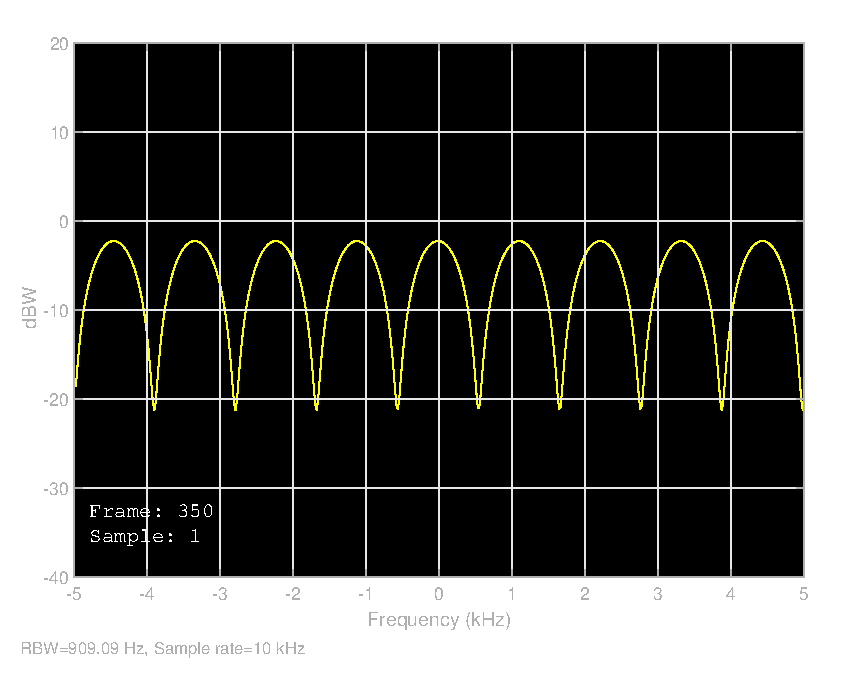
\includegraphics[width=0.5\textwidth]{FlatFadingFrequencyResponse}
				\caption{Figure showing the frequency when I run the flat fading model}
				\label{fig:FlatFadingFreqResp}
			\end{figure}
			\begin{figure}
				\centering
				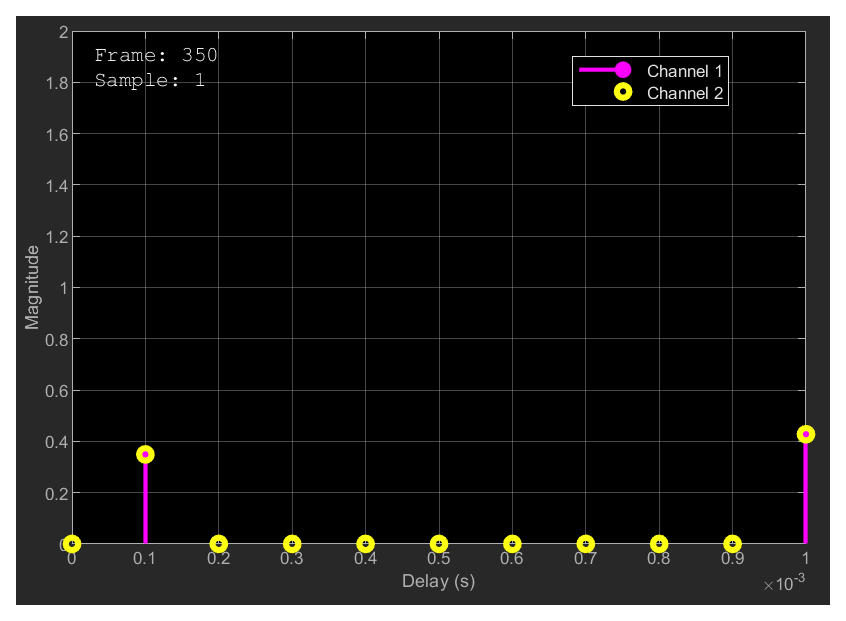
\includegraphics[width=0.5\textwidth]{FlatFadingImpulseResponse}
				\caption{Figure showing the impulse when I run the flat fading model}
				\label{fig:FlatFadingImplResp}
			\end{figure}
		}
		\subsection{Frequency Selective Fading}
		{
			Frequency Selective Fading occurs when $B_S > B_C$ and $T_S < \sigma_\tau$ Lets start with the $B_S > B_C$:
			\subsubsection{\texorpdfstring{$B_S > B_C$}{}}
			{
				\label{sec:BS>BC}
				This means the signal bandwidth is greater than the coherence bandwidth. This can be achieved by setting the output of the binary generator to output at $10^4$ bits per second and the coherence bandwidth can be set as it is approximately $\frac{1}{\tau_{max}}$ Therefore all we need to do is set $\tau_{max}$ to less than $10^{-4}$(As it is inverted) therefore well set it to $10^{-5}$.
			}
			\subsubsection{\texorpdfstring{$T_S < \sigma_\tau$}{}}
			{
				This means the Symbol period is less than the RMS delay spread the symbol period set in \cref{sec:BS>BC} which is $10^{4}$ symbols per second. so the RMS delay spread has to be more that the $10^{-4}$. The inputs I set for this can be found in \cref{img:FreqSelectFadeSISOParams}. From my calculations this gives us an RMS delay spread of $5\times10^{-4}$ 
				\begin{figure}
					\centering
					\includegraphics[width=0.5\textwidth]{FrequencySelectiveFadingSISOFadingParameters}
					\caption{Parameters for SISO fading channel to set RMS Delay spread}
					\label{img:FreqSelectFadeSISOParams}
				\end{figure}
			}
			\begin{figure}
				\centering
				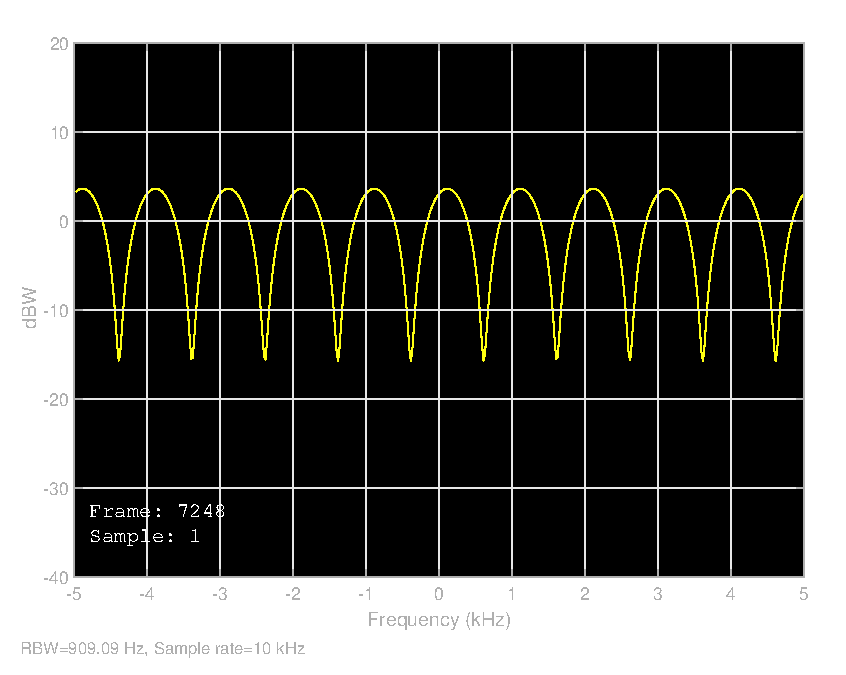
\includegraphics[width=0.5\textwidth]{SelectiveFadingFrequencyResponse}
				\caption{Figure showing the frequency when I run the selective fading model}
				\label{fig:SelectFadingFreqResp}
			\end{figure}
			\begin{figure}
				\centering
				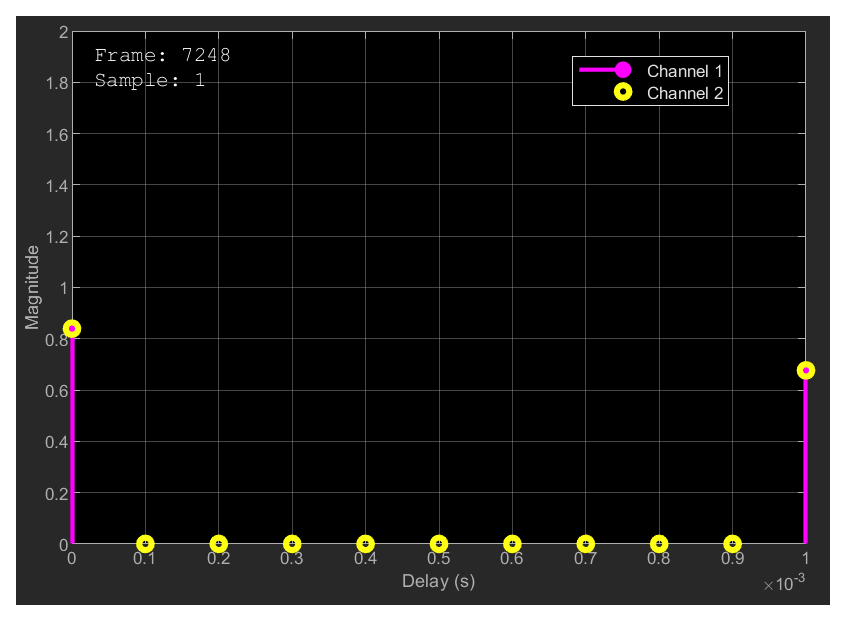
\includegraphics[width=0.5\textwidth]{SelectiveFadingImpulseResponse}
				\caption{Figure showing the impulse when I run the selective fading model}
				\label{fig:SelectFadingImplResp}
			\end{figure}
			\Cref{fig:SelectFadingFreqResp} and \cref{fig:SelectFadingImplResp} show the outputs from the Simulink model when I run the selective frequency model with the inputs mentioned above.
		}
		\subsection{Slow Fading}
		{
			
		}
		\subsection{Fast Fading}
		{
			
		}
	}
	\section{Conclusion}
	{
		
	}
	
	
	\newpage
	
	\printbibliography[heading=bibintoc,title=References]
\end{document}
